\section{Evaluation}
\label{sec:results}
In this section, we conduct a thorough design space exploration to verify the effectiveness of the proposed LatentMoE architecture. We start by pretraining Transformer MoE models at two different scales: (1) 16B total parameters with 2B active, which we use for conducting ablation studies, and (2) 95B total parameters with 8B active, which we use as a scaling test of the 16B results. To demonstrate the generalizability of LatentMoE architectures, we further extend our study by training hybrid Mamba-Attention MoE models at scale. 

We use the architecture and hyperparameters from DeepSeek-v2-lite~\citep{deepseek_v2} for our 2B active model ablations. For the 8B active Transformer model, we use a cosine learning rate schedule with a max learning rate of $1.2 \times 10^{-3}$ decayed to a minimum of $3 \times 10^{-6}$. The 8B active Hybrid model is trained with a WSD schedule with a max learning rate of $8 \times 10^{-4}$ decayed to $8 \times 10^{-6}$ in the last 15\% of training.  Both the 8B active Transformer and hybrid models are trained with a sequence length of 8192, a batch size of 768 ($\sim6$ million tokens), and a learning rate warmup of $8.4$ billion tokens. The 8B active models use a load balancing loss coefficient of $10^{-4}$ along with DeepSeek’s aux-loss-free load balancing strategy~\citep{auxiliarylossfreeloadbalancingstrategy} to ensure balanced token load throughout training. Table~\ref{tbl:model_arch} summarizes the model architecture under study in this paper. 

\begin{table}[ht!]
    \centering
    \caption{Architectural specifications of the baseline models used for design space exploration. For the Hybrid model's Mamba layers, we use Mamba-2 blocks with 128 heads, 64 head dimension, 128 state dimension, and 8 groups.}
    \label{tbl:model_arch}
    \resizebox{\textwidth}{!}{%
    \begin{tabular}{lccc}
    \toprule
    \textbf{Configuration} & \textbf{16BT-2BA} & \textbf{95BT-8BA} & \textbf{Hybrid-73BT-8BA} \\
    \midrule
    Layers ($L$) & 27 & 32 & 52 (24 Mamba/MoE, 4 Attn.)\\
    Hidden Dimension ($d$) & 2048 & 4096 & 4096\\
    Total Routed Experts ($N$) & 64 & 128 & 128 \\
    Active Experts ($K$) & 6 & 6 & 6 \\
    Shared Experts ($S$) & 2 & 2 & 2 \\
    Intermediate FFN Dimension ($m$) & 1408 & 2688 & 2688 \\
    Activation Function & SwiGLU & Squared-ReLU & Squared-ReLU \\
    Attention Heads & 16 & 32 & 32 \\
    Query Groups (GQA) & 16 & 8 & 8 \\
    \midrule
    Total Parameters & 16B & 95B & 73B \\
    Active Parameters & 2B & 8B & 8B \\
    \bottomrule
    \end{tabular}
    }
\end{table}

\subsection{LatentMoE Ablations}

\newparagraph{Impact of compression ratio.} Design Principle IV (Section~\ref{sec:design_choices}) hypothesizes that there exists an intrinsic rank $r_{\mathrm{eff}}$ such that compressing the latent dimension to $\ell \ge r_{\mathrm{eff}}$ results in negligible information loss. To empirically validate this and estimate $r_{\mathrm{eff}}$, we pretrain and sweep different compression ratios on top of the $\lmoeeff$ configuration, holding all other hyperparameters constant.
Results in Figure~\ref{fig:results_2b_vary_compression} indicate that model quality is preserved for compression ratios $\alpha \le 4$. Consequently, we adopt $\alpha = 4$ for all subsequent experiments. We empirically verified that this setting remains effective at larger scales as well (i.e., 95B total and 8B active).

\begin{figure}[ht!]
    \centering
    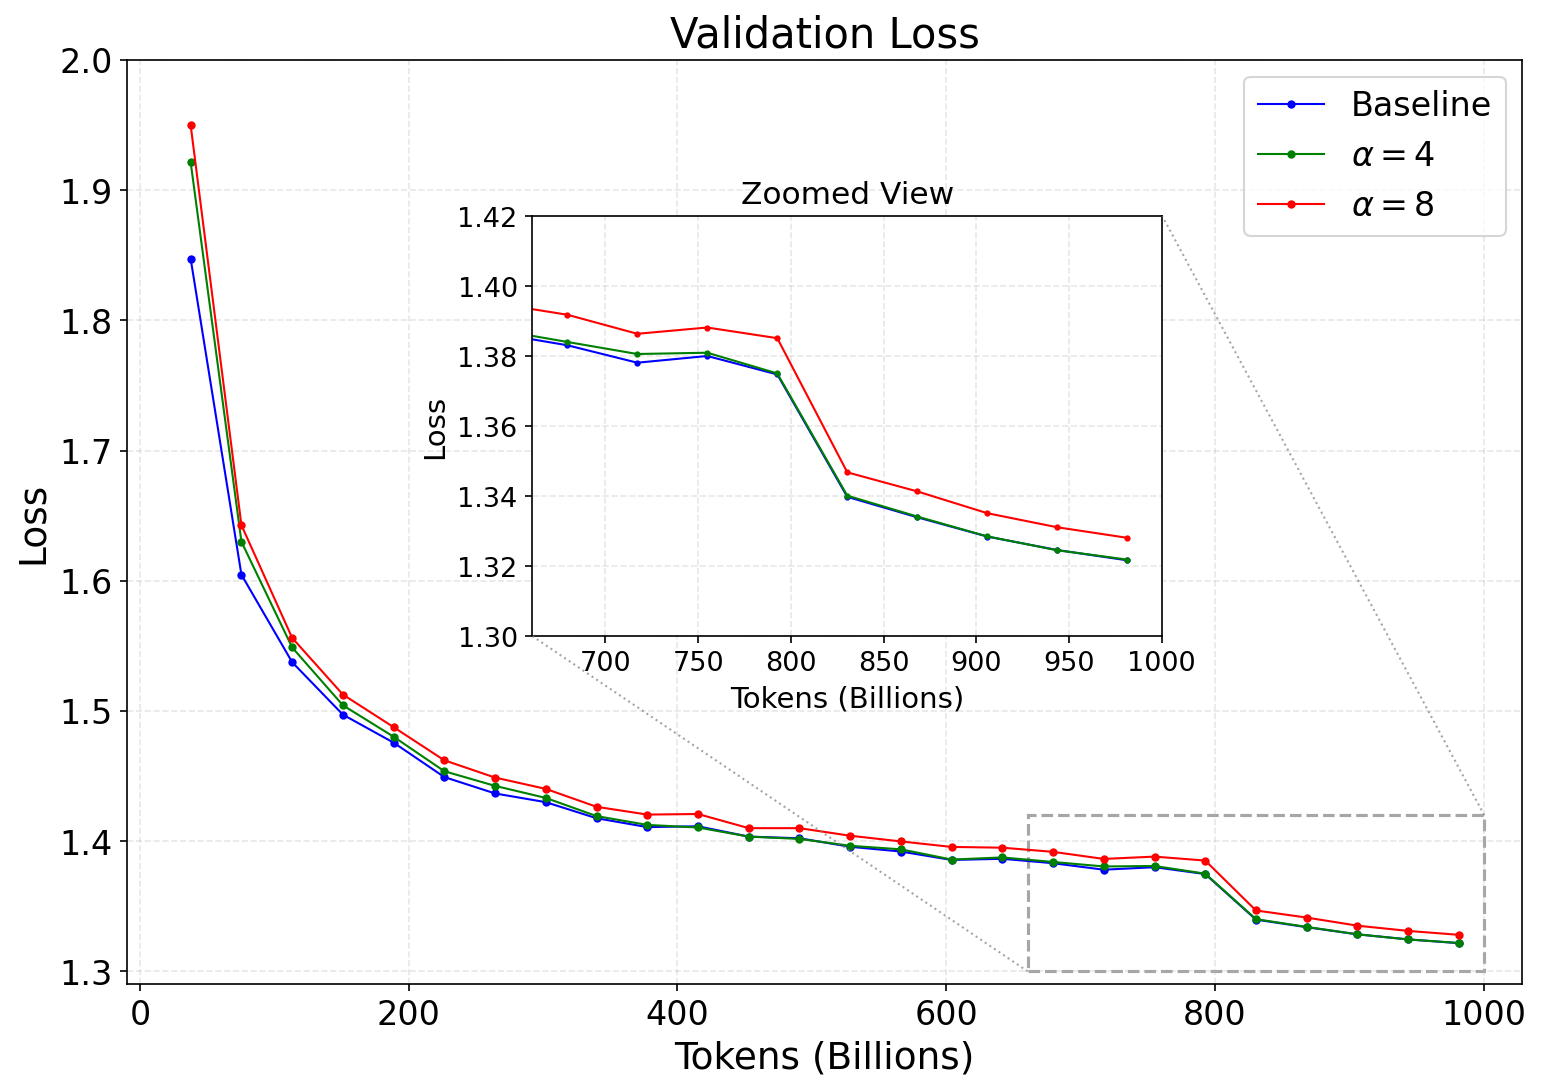
\includegraphics[width=0.7\textwidth]{figures/2B_vary_alpha_lmoe_eff.png}
    \caption{\textbf{Effect of compression ratio on model quality.} Validation loss for the 16BT-2BA model using the $\lmoeeff$ configuration across varying compression ratios $\alpha=d/\ell$. The total number of experts is scaled by $\alpha$, while the base model configuration follows Table~\ref{tbl:model_arch}.}
    \label{fig:results_2b_vary_compression}
\end{figure}


\begin{figure}[ht!]
    \centering
    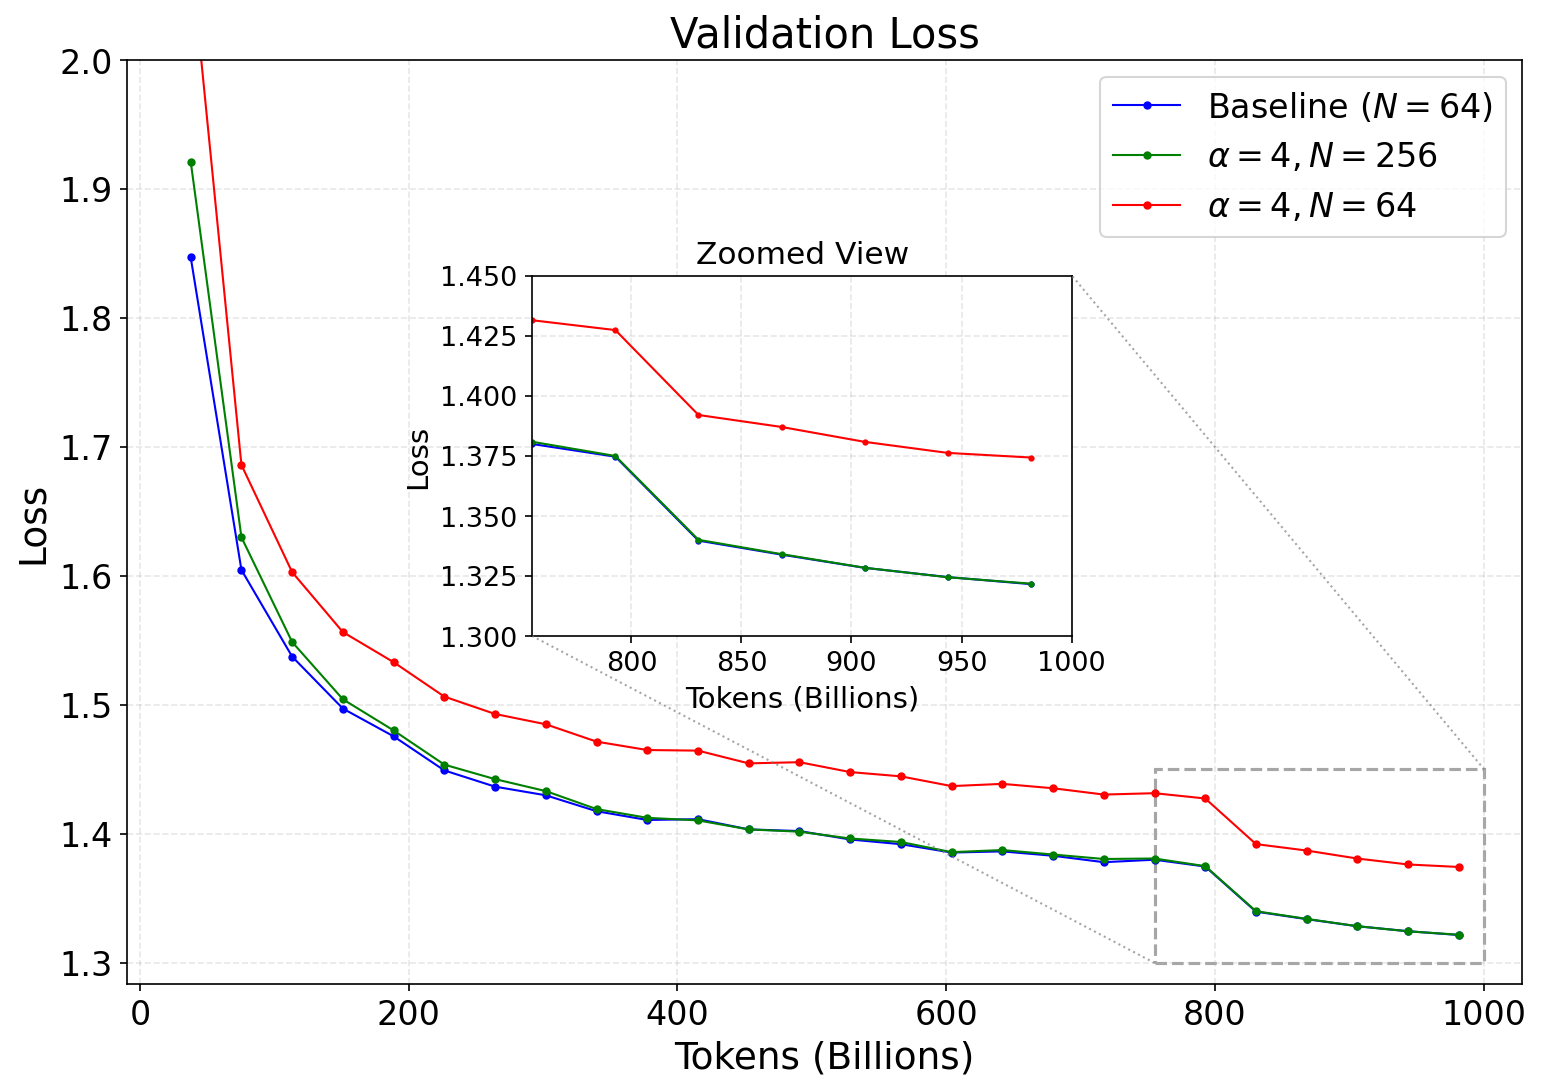
\includegraphics[width=0.7\textwidth]{figures/2B_reduced_params.png}
    \caption{\textbf{Impact of expert scaling on model quality.} Comparison of validation loss for the 16BT-2BA model using the $\lmoeeff$ configuration when the hidden dimension is compressed by $4\times$. The green curve utilizes the proposed expert scaling ($N' = \alpha N$), while the red curve does not. Scaling the expert count effectively mitigates the accuracy loss caused by compression, eliminating the need for extensive hyperparameter retuning.}
    \label{fig:results_reduced_params}
\end{figure}

\newparagraph{Impact of number of experts.}
In Section~\ref{sec:latentmoe}, we noted that parameter reduction via compression can impede training stability. To quantify this, we pretrain the $\lmoeeff$ LatentMoE variant of the 16B total and 2B active parameter model with the hidden dimension $d$ compressed by a factor of 4, both with and without a compensatory increase in the total number of experts, using the baseline hyperparameters. As shown in Figure~\ref{fig:results_reduced_params}, reducing $d$ without scaling the expert count leads to significant quality degradation, validating the expert scaling strategy employed by LatentMoE.


\newparagraph{Comparison between the two variants of LatentMoE.}
In Section~\ref{sec:latentmoe}, we introduced two LatentMoE variants: $\lmoeeff$, designed to improve inference efficiency while maintaining baseline accuracy, and $\lmoeacc$, designed to enhance accuracy at a comparable inference cost. Figure~\ref{fig:results_2b_latent512_baseline_leff_lacc} compares the validation loss of these configurations against the baseline for the 16B total and 2B active parameter model using a latent dimension of $\ell=512$ ($\alpha=4$). Consistent with our expectations, $\lmoeeff$ matches the baseline accuracy, whereas $\lmoeacc$ achieves a noticeably lower validation loss. \textcolor{green!50!black}{\textit{We recommend $\lmoeacc$ for Pareto-optimal accuracy versus inference cost.}} \\

\begin{figure}[h]
\centering
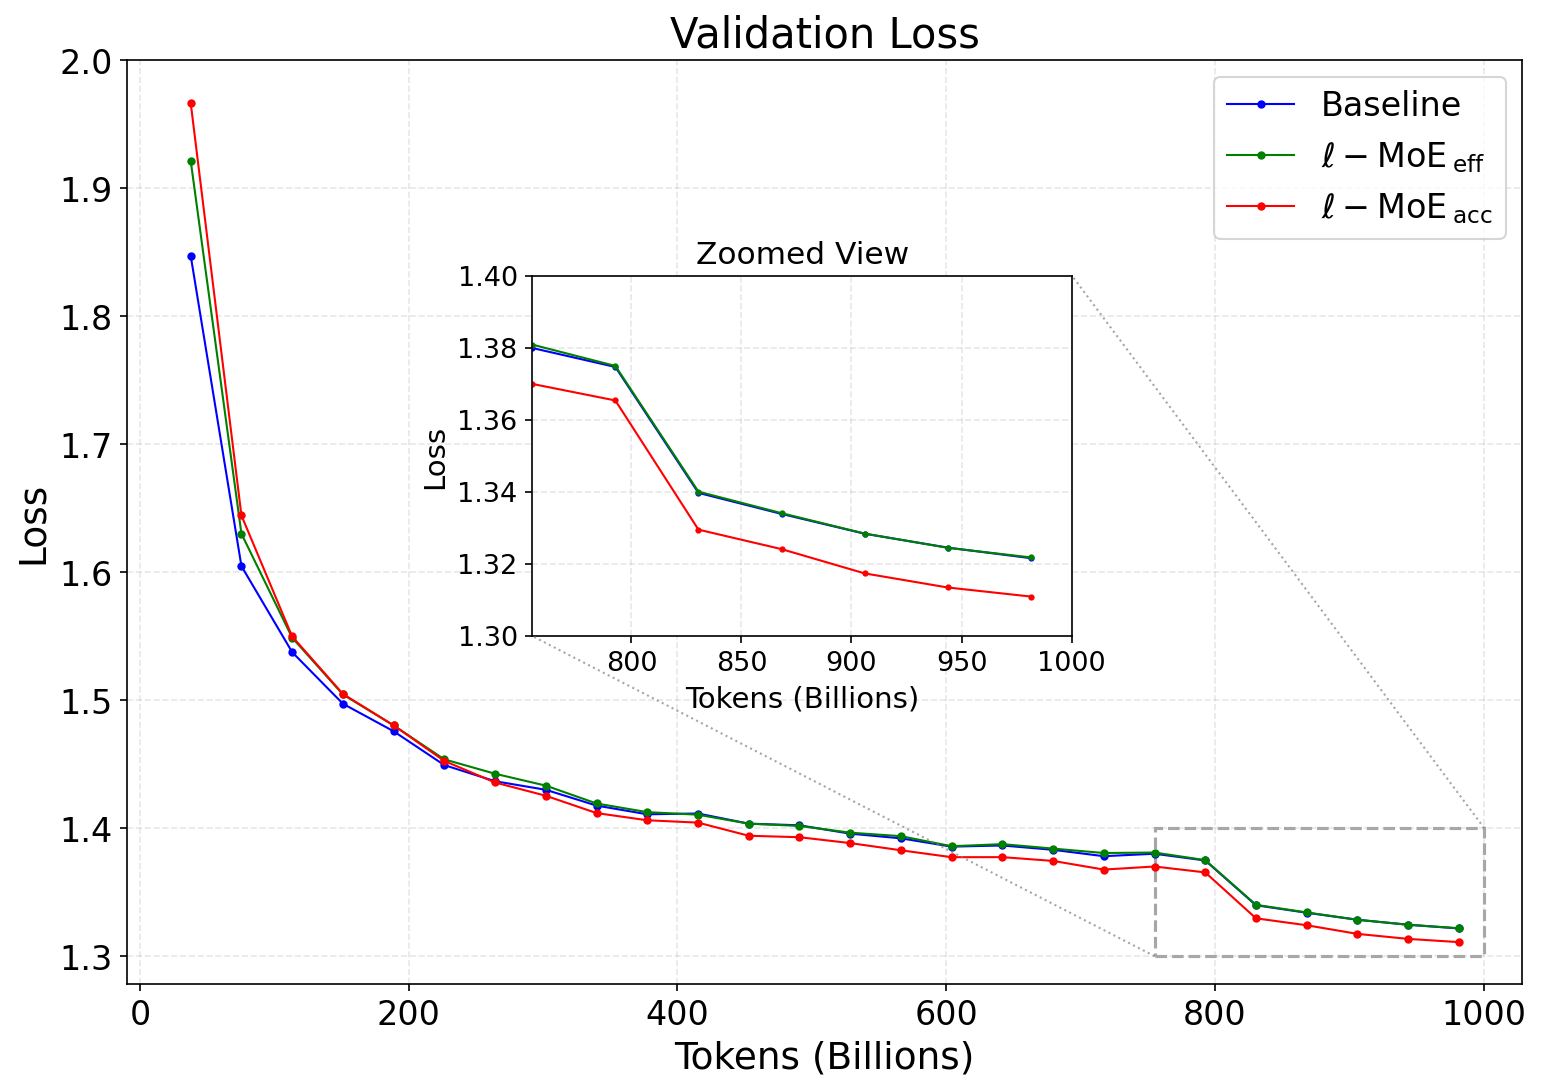
\includegraphics[width=0.7\textwidth]{figures/2b_latent512_baseline_leff_lacc.png}
\caption{\textbf{Comparison between LatentMoE variants.} Training trajectories for the baseline 16BT-2BA
model versus the $\lmoeeff$ and $\lmoeacc$ ($\ell=512$). $\lmoeeff$ matches baseline convergence, while $\lmoeacc$ outperforms the baseline. }
\label{fig:results_2b_latent512_baseline_leff_lacc}
\end{figure}


\subsection{LatentMoE Scaling Studies}
\label{sec:accuracies}
Leveraging the insights from the 16B model ablations, we train a 95B parameter Transformer using a LatentMoE configuration with a $4\times$ compression ratio. Figure~\ref{fig:8b_val_loss} presents the validation loss trajectories for $\lmoeeff$ and $\lmoeacc$ relative to the baseline. Consistent with the 16BT-2BA results, $\lmoeeff$ matches the baseline, while $\lmoeacc$ demonstrates superior results. Table~\ref{tbl:8b_acc} shows the downstream task accuracy at the 300B token horizon.
We report Code as the average over HumanEval, HumanEval+, MBPP, and MBPP+, Math as the average of GSM8K CoT and MATH-500, and Commonsense understanding as the average of RACE, ARC-Challenge, HellaSwag, and Winogrande.
For simplicity, we used the exact same hyperparameters optimized for the baseline Transformer for LatentMoE. Further hyperparameter tuning might lead to even better accuracy.

\begin{figure}[ht!]
\centering
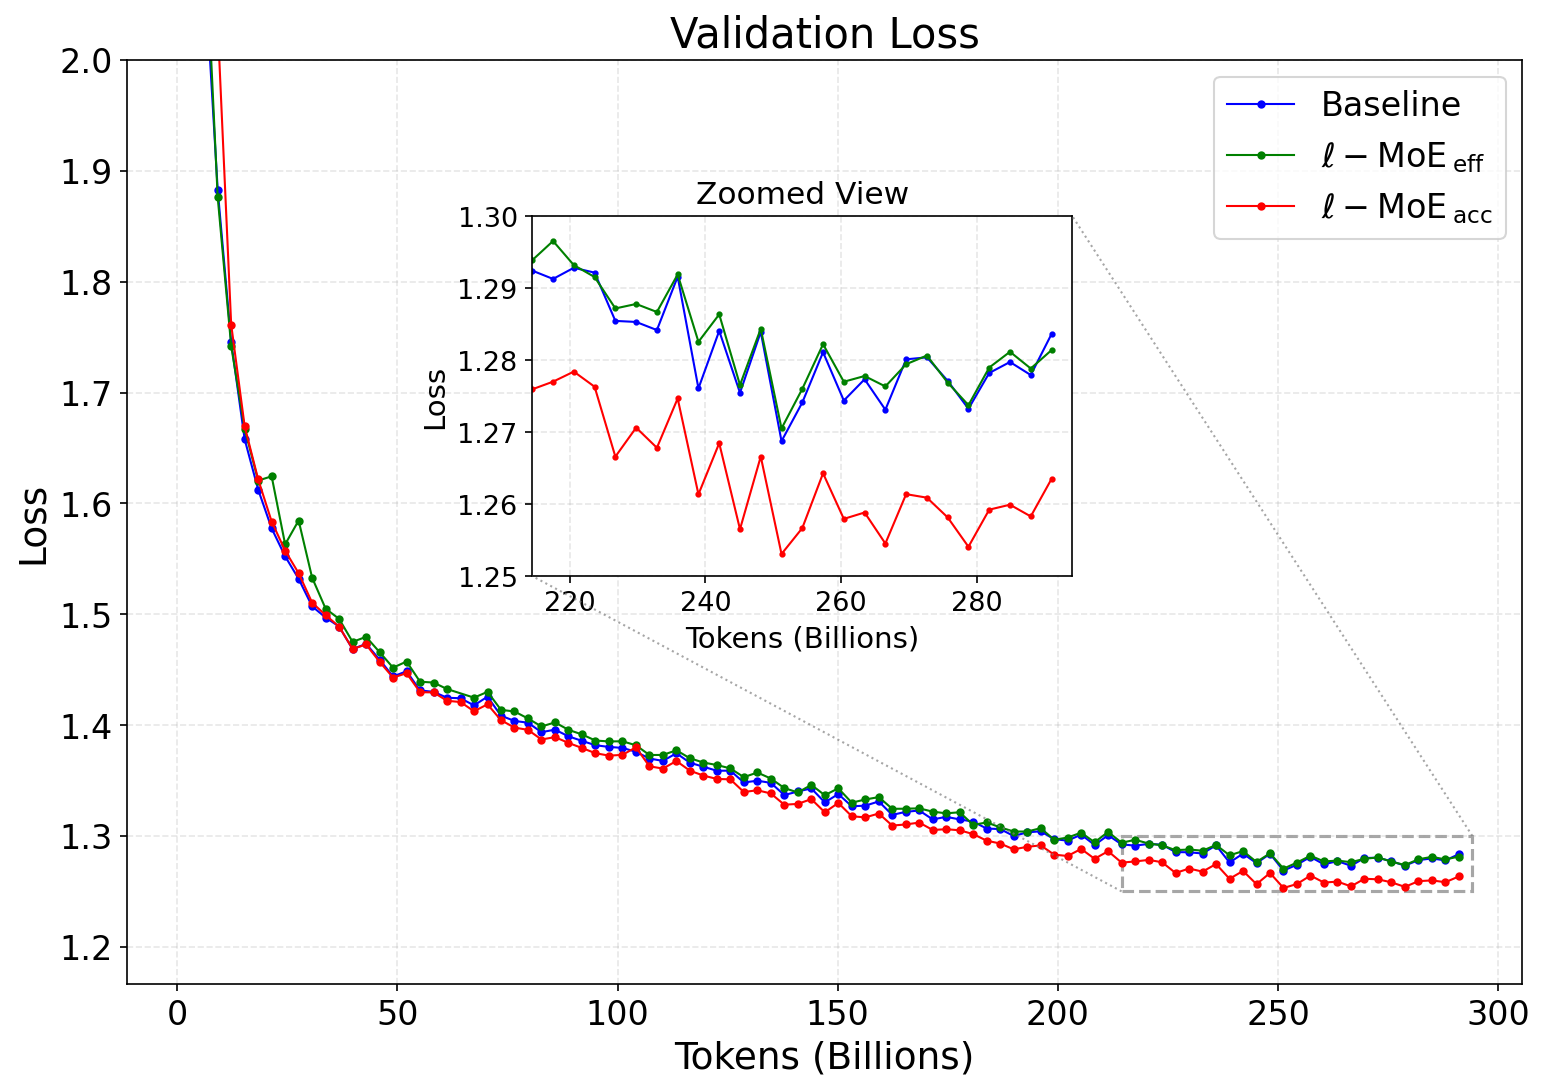
\includegraphics[width=0.7\textwidth]{figures/8B_val_loss.png}
\caption{\textbf{95B Model Training Convergence.} Validation loss curves for the 95BT-8BA baseline, $\lmoeeff$, and $\lmoeacc$ configurations ($\ell=1024, \alpha=4$). $\lmoeeff$ matches baseline convergence, while $\lmoeacc$ outperforms the baseline.}
\label{fig:8b_val_loss}
\end{figure}

\begin{table}[ht!]
    \centering
    \caption{Accuracy comparisons of the 95BT-8BA model with and without LatentMoE. Compared to the baseline, with equivalent parameters, $\lmoeacc$ provides higher accuracy across all downstream tasks, while $\lmoeeff$ provides comparable to or better accuracy with much fewer FLOPs.}
    \label{tbl:8b_acc}
    \resizebox{\textwidth}{!}{%
    \begin{tabular}{lccccccc}
    \toprule
    \textbf{Model} & \textbf{Active Params} & \textbf{Total Params} & \textbf{MMLU Pro} & \textbf{MMLU} & \textbf{Code} & \textbf{Math} & \textbf{Commonsense} \\
    \midrule
    Baseline & 8.47B & 94.4B & 29.26 & 58.95 & 40.33 & 64.39 & 74.32 \\
    \midrule
    $\lmoeacc$ & 8.44B & 94.8B & \textbf{34.91} & \textbf{62.23} & \textbf{41.50} & \textbf{64.88} & \textbf{75.18} \\
    $\lmoeeff$ & 5.62B & 94.8B & 34.75 & 61.06 & 40.68 & 63.61 & 73.72 \\
    \bottomrule
    \end{tabular}
    }
\end{table}


To further validate the effectiveness of the LatentMoE architecture, we also pretrain a series of hybrid Mamba-Attention MoE models. Specifically, we first train a baseline 8B active (73B total) parameter model. As described in Table~\ref{tbl:model_arch}, each MoE layer in the hybrid architecture contains 128 experts, 6 activated experts, 2 shared experts, and uses an intermediate FFN dimension of 2688. We use Squared-ReLU activation and a model dimension of 4096. We then train the $\lmoeeff$ and $\lmoeacc$ LatentMoE variants of the baseline model, using a $4\times$ compression ratio.

Results after training the above models on 1T tokens are shown in Table~\ref{tbl:hybrid_8b_1t}. All models are trained with identical hyperparameters. As shown, the LatentMoE $\lmoeacc$ variant achieves significantly higher accuracy than the baseline across all tasks, while the $\lmoeeff$  variant achieves accuracy comparable to or better than the standard granular MoE baseline. 

Overall, the LatentMoE architecture provides a clear advantage in terms of accuracy per FLOP and per parameter compared to granular MoEs, paving the way for higher accuracy at fixed inference cost or lower inference cost at fixed accuracy.

\begin{table}[h]
    \centering
    \caption{Accuracy comparisons of hybrid Mamba-Attention MoEs with and without LatentMoE. Compared to the baseline, with equivalent parameters, $\lmoeacc$ provides higher accuracy across all downstream tasks, while $\lmoeeff$ provides comparable or better accuracy with much fewer FLOPs.}
    \label{tbl:hybrid_8b_1t}
    \resizebox{\textwidth}{!}{%
    \begin{tabular}{lccccccc}
    \toprule
    \textbf{Model} & \textbf{Active Params} & \textbf{Total Params} & \textbf{MMLU Pro} & \textbf{MMLU} & \textbf{Code} & \textbf{Math} & \textbf{Commonsense} \\
    \midrule
    Baseline & 8.09B & 72.6B & 48.30 & 70.10 & 51.95 & 78.32 & 81.73 \\
    \midrule
    $\lmoeacc$ & 8.02B & 72.8B & \textbf{52.87} & \textbf{72.11} & \textbf{55.14} & \textbf{80.19} & \textbf{82.10} \\
    $\lmoeeff$ & 5.91B & 72.8B & 51.29 & 71.34 & 53.13 & 77.01 & 80.78 \\
    \bottomrule
    \end{tabular}
    }
\end{table}


\subsection{Inference Performance}
As discussed in Section~\ref{sec:latentmoe}, $\lmoeacc$ is expected to achieve similar inference speed to the standard MoE baseline while attaining higher accuracy.
Our evaluations in Section~\ref{sec:accuracies} confirmed that $\lmoeacc$ indeed achieves higher accuracy compared to standard MoE. Here, we evaluate $\lmoeacc$ from the perspective of inference efficiency.
Table~\ref{tbl:measuredperf} presents the measured performance of $\lmoeacc$ compared to standard MoE for the Hybrid-73BT-8BA model (see Table~\ref{tbl:model_arch}) on two Hopper H100 GPUs using vLLM with FP8 per-tensor quantization.
We focus our measurements on the hybrid Mamba-Attention baseline, as it represents the most efficient inference architecture.

\begin{table}[ht!]
    \centering
    \footnotesize
    \begin{tabular}{ccc}
    \hline
     \textbf{Concurrency} & \textbf{LatentMoE (Tokens/s/GPU)} & \textbf{Standard MoE (Tokens/s/GPU)} \\
    \hline
   1 & 181.6 & 206.6 \\
     4 & 528.5 & 509.8 \\
    16 & 1130.8 & 1204.6 \\
     64 & 1569.6 & 1549.3 \\
     128 & 1625.8 & 1725.9 \\
    \hline
    \end{tabular}
    \caption{Comparison of LatentMoE and Standard MoE performance metrics.}
    \label{tbl:measuredperf}
\end{table}

The measurements show that at higher concurrencies, per-GPU throughput drops by only up to 6\%. It is important to note that further software optimizations could be performed to mitigate even these small throughput differences between LatentMoE and standard MoE. One proposed optimization is to utilize separate CUDA streams for routed and shared experts, which could reduce end-to-end latency when performing inference with smaller batches or when model dimensions do not saturate the GPU's compute. A second optimization targets the MoE kernels from the CUTLASS library. Since LatentMoEs decrease the size of the GEMMs for routed experts, it is important to ensure that inner dimensions remain large enough to fully utilize the GPU and avoid SM-bound workloads. When inner dimensions are small, specialized smaller-matrix GEMM kernels should be used.


\subsubsection{Projected Serving Impact at Trillion-Parameter Scale}
\label{sec:discussion_projected_serving} 

Inference efficiency can be characterized as a three-dimensional trade-off surface, with accuracy along one axis, throughput per GPU along a second axis, and latency (user interactivity) along the third axis. Thus far, we have discussed the accuracy of LatentMoE and presented measured performance at the 95B-parameter scale. In the following section, we examine a two-dimensional slice of this trade-off at the trillion-parameter scale by projecting throughput per GPU and latency Pareto frontiers for accuracy-matched models.

\begin{figure}[ht!]
  \centering
  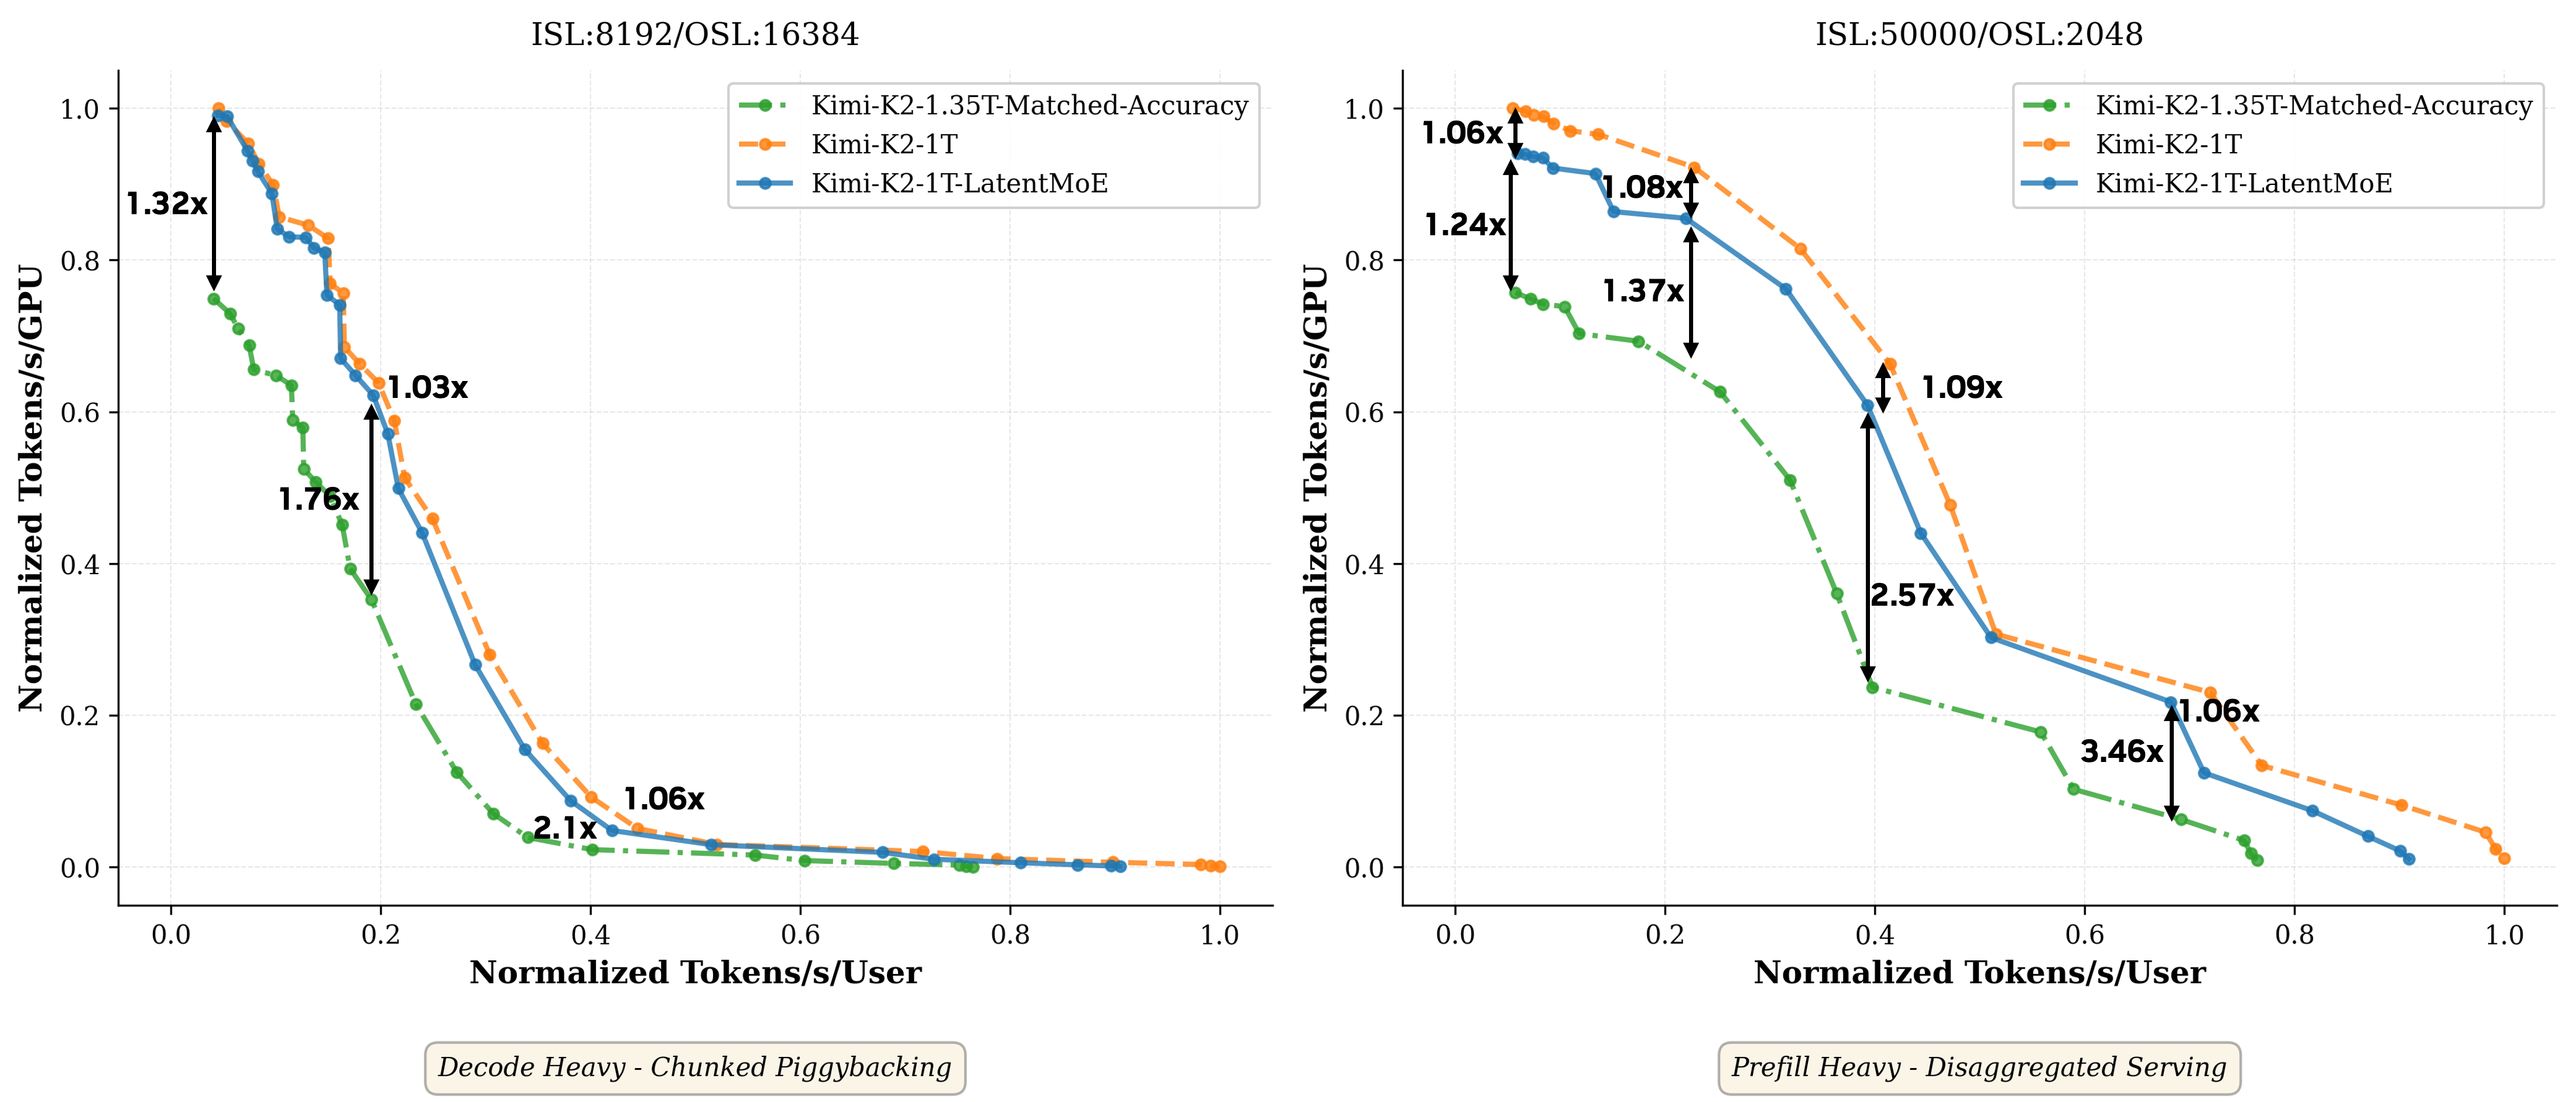
\includegraphics[width=1.0\linewidth]{figures/normalized_plot.png}
  \caption{\textbf{Projected throughput-latency Pareto frontiers at trillion-parameter scale.}
  \textit{Left:} Decode-heavy traffic modeled with chunked piggybacking serving. \textit{Right:} Prefill-heavy traffic modeled with disaggregated serving.
  \textsc{Kimi-K2-1T-LatentMoE} attains accuracy-efficient operating points. Matching its accuracy under standard MoE scaling requires an additional $\sim$350B parameters in our construction and yields a $1.24\times$--$3.46\times$ projected slowdown across the frontier.}
  \label{fig:normalized_plot}
\end{figure}

\noindent \textbf{Performance evaluation methodology.} We use a high-fidelity proprietary performance simulator to project end-to-end serving performance for a trillion-parameter class model and its LatentMoE variant. We simulate over $200$K operating points to estimate the throughput per GPU and latency Pareto frontiers shown in Figure~\ref{fig:normalized_plot}. We consider two traffic patterns. The first is a decode-heavy setting modeled with chunked piggybacking serving. The second is a prefill-heavy setting modeled with disaggregated serving, where prefill and decode are separated to reflect long-context traffic. The serving strategy (for example, whether to use disaggregation) is selected following the guidance in~\cite{mitra2025beyond}.

\noindent \textbf{Effective Parameter Multiplier (EPM).} We use the effective parameter multiplier to construct an iso-accuracy baseline for inference comparisons. We benchmark the native \textsc{Kimi-K2-1T} against our proposed variant, \textsc{Kimi-K2-1T-LatentMoE}. Following the ``Effective Parameter Count'' framework established by~\cite{frantar2025compressionscaling}, we posit that a treated model with physical parameters $N_{treat}$ behaves like a standard dense baseline with effective parameters $N_{eff}$. We assume baseline performance follows a scaling law $f(N)$. For a treated model achieving score $S_{treat}$, the effective capacity is obtained by inverting the baseline scaling law:
\begin{equation}
    N_{eff} = f^{-1}(S_{treat})
\end{equation}
The EPM is defined as the ratio of effective capacity to physical parameters:
\begin{equation}
    \lambda = \frac{N_{eff}}{N_{treat}}
\end{equation}
We use $\lambda$ to construct an iso-accuracy baseline with parameter count $N_{\text{iso}} = \lambda \cdot N_{treat}$. For our evaluations, we derive $f(N)$ by fitting a log-linear function to the MMLU accuracy scores of the \textsc{Qwen-3-Dense} model family (0.6B, 1.7B, 4B, 8B, 14B, and 32B):
\begin{equation}
    f(N) = a \cdot \log N + b
\end{equation}
where $a$ and $b$ are fitted parameters.

\noindent \textbf{Iso-accuracy baseline construction.} We estimate an Effective Parameter Multiplier of $\lambda \approx 1.35\times$ for \textsc{Kimi-K2-1T-LatentMoE}. For a 1T-parameter base model, this implies an iso-accuracy scale of $N_{\text{iso}} \approx 1.35$T, corresponding to an increase of $(1.35 - 1.0)$T $\approx 0.35$T $\approx 350$B parameters. Guided by this target, we construct a physical \textbf{iso-accuracy baseline}, denoted \textsc{Kimi-K2-1.35T}, by scaling the native architecture depth from 61 to 80 layers. This construction matches the projected effective capacity implied by LatentMoE and enables a direct inference-efficiency comparison against a standard model of comparable predictive power.

\noindent \textbf{Accuracy matching with standard MoE scaling is more expensive.} $\lmoeacc$ achieves an accuracy gain at fixed parameter and FLOP budget. When we enforce an accuracy-matched comparison using the standard MoE architecture, the required scaling incurs a marked serving penalty. Across the projected Pareto frontier (Figure~\ref{fig:normalized_plot}), \textsc{Kimi-K2-1.35T} is approximately $1.24\times$--$3.46\times$ slower than \textsc{Kimi-K2-1T-LatentMoE}, indicating that $\lmoeacc$ provides a more favorable accuracy-latency trade-off than increasing model size through the standard MoE architecture to reach the same accuracy target.

\noindent \textbf{Latent projection overhead is modest.} Relative to native \textsc{Kimi-K2-1T}, \textsc{Kimi-K2-1T-LatentMoE} introduces additional computation due to latent projection operators. In our projections, native \textsc{Kimi-K2-1T} remains close, within up to $\sim$9\% of \textsc{Kimi-K2-1T-LatentMoE}, indicating that projection overhead is small compared to the cost of achieving the same accuracy gain via standard scaling to \textsc{Kimi-K2-1.35T}.
